% !TeX encoding   = UTF-8
\documentclass[12pt]{article}

\usepackage{sbc-template}

\usepackage{graphicx,url}
\usepackage[brazil]{babel}
\usepackage[utf8]{inputenc}
\usepackage{graphicx}   %Package para figuras
\usepackage{enumerate}
\usepackage{tabularx}
\usepackage{multirow}
\usepackage[table,xcdraw]{xcolor}
\usepackage{todonotes}

\sloppy

\title{Um estudo sobre o efeito de Mover Classe na Arquitetura de Sistemas}

\author{Vagner Clementino\inst{1}}

\address{Departamento de Ciência da Computação\\
        Universidade Federal de Minas Gerais (UFMG)\\
  \email{vagnercs@dcc.ufmg.br}
}

\date{Maio de 2016}
\begin{document}

\maketitle

%\begin{abstract}
%  This meta-paper describes the style to be used in articles and short papers
%  for SBC conferences. For papers in English, you should add just an abstract
%  while for the papers in Portuguese, we also ask for an abstract in
%  Portuguese (``resumo''). In both cases, abstracts should not have more than
%  10 lines and must be in the first page of the paper.
%\end{abstract}

\begin{resumo}
 \textbf{TODO}
\end{resumo}


\section{Introdução}
\label{sec:intro}

A atividade de refatoração tem por objetivo alterar o código fonte de um software sem modificar o seu comportamento. Em última instância, refatorar visa melhorar a qualidade interna do sistema \cite{Fowler1999,Opdyke:1992:ROF:169783}. Sua importância é reconhecida tanto na literatura quanto na indústria, no qual, nesta última, é possível verificar a existência de processos de desenvolvimento que incorporam a refatoração como atividade rotineira \cite{Beck:2000:PEP:557458}. No últimos anos, pesquisas foram realizadas com o objetivo de entender com qual frequência os desenvolvedores aplicam os diferentes tipos de refatoração \cite{Murphy-Hill:2009:WRW:1555001.1555044}; a relação entre a atividade de refatorar e a correção de \textit{bugs}\cite{Kim:2011:EIR:1985793.1985815} bem como nos resultados de testes de regressão  \cite{Kim:2012:EII:2473496.2473590}. No trabalho de kim et.al discute a percepção dos desenvolvedores sobre a refatoração \cite{Kim:2012:FSR:2393596.2393655}.

Recentemente estudos vêm focando em entender as motivações que levam os desenvolvedores a realizem refatoração. Existe um consenso que a motivação original é remover porções de código com baixa qualidade conhecidos como \textit{Bad Smells} \cite{Fowler1999}. Todavia, estudos demonstraram que o desenvolvedores refatoram para outros fins, como por exemplo, a refatoração \textit{Extrair Método}  pode ser utilizada para fins de extensão do sistema ou mesmo possibilitar compatibilidade com versões anteriores do código \cite{Tsantalis2013}. É possível verificar a utilização do \textit{Extrair Método} visando favorecer a reutilização de código no longo prazo,mesmo que inicialmente não seja esta a intenção \cite{Danilo}.

Apesar da existência de estudos relativos à motivação da refatoração, ao bem do nosso conhecimento, não existem trabalhos que relacionem a refatoração \textit{Mover Classe} com mudanças na arquitetura do sistema. Suspeitamos que o fato de um desenvolvedor mover classes em um número maior que padrão do sistema tem por objetivo alterar a arquitetura do sistema. Este tipo de ação é conhecida como \textit{batching moving}. A mudança na arquitetura pode ter como objetivo, por exemplo, reorganizar o código existente em uma nova camada lógica ou ainda tratar o problema da  \textit{Erosão Arquitetural}. O processo de Erosão arquitetural é conhecido como os desvios ocorridos no código de um sistema que causam violação de alguma regra arquitetural previamente estabelecida\cite{Perry:1992:FSS:141874.141884}.

Neste sentido, este trabalho se propõe em analisar a relação entre mudanças na arquitetura de um sistema e a refatoração \textit{Mover Classe}. A fim de investigar tal relação analisamos o histórico de versões de 04 sistemas de código aberto \todo{Listar os sistemas escolhidos} desenvolvidos em Java e procedemos com um \textit{survey} com os desenvolvedores visando responder as seguintes questões de pesquisa:

\begin{description}
	\item[RQ1] Com qual frequência a refatoração Mover Classe tem por objetivo alterar a arquitetura do sistema (\texttt{batching moving})?
	\item[RQ2] Com qual frequência o desenvolvedor informa no \textit{log de commit} que a refatoração teve por objetivo alterar a arquitetura do sistema?
	\item[RQ3] Segundo dos desenvolvedores, Mover Classe foi efetivamente utilizado para alterar a arquitetura dos sistema?	
\end{description}

Ao responder as questões proposta neste trabalho entendemos que iremos contribuir no aumento do entendimento das razões que levam os desenvolvedores a realizar refatorações. Esta informação poderá ser utilizada posteriormente na construção de ferramentas que ajudem os times de desenvolvimento em tarefe relativas à mudança da arquitetura do software. Além disso será possível verificar a relação entre a atividade de refatoração e a mudança de arquitetura de um sistema. 

O restante deste trabalho está organizado da seguinte forma: a Seção \ref{sec:metodologia} descreve a metodologia utilizada neste estudo; a Seção \ref{sec:resultados} apresenta os resultados e responde as questões de pesquisas propostas; na Seção \ref{sec:ameacas} realiza-se uma discussão sobre as ameaças à validade do trabalho; a Seção \ref{sec:trabalhos-relacionados} apresenta os trabalhos relacionados à análise da atividade e detecção de refatoração; a Seção \ref{sec:conclusao} sumariza o artigo e discute suas principais contribuições.

\section{Metodologia}
\label{sec:metodologia}


\subsection{Seleção dos Sistemas}
\label{subsec:selecao_sistemas}

Com o objetivo de responder as questões de pesquisa propostas neste trabalho foram coletados sistemas de código aberto hospedados no \textsl{GitHub}. Com cerca de 38 milhões de repositórios\footnote{\url{https://github.com/features}. Acesso em junho/2016.}, GitHub é atualmente o maior repositório de código on line do mundo. Sua popularidade e a disponibilidade de metadados acessíveis através de uma API tem tornando GitHub bastante atrativo para a realização de pesquisas na área de Engenharia de Software. 

Para escolha dos projetos foi definido inicialmente um conjunto de critérios que foram baseados em boas práticas recomendadas na literatura\cite{Bird2009}. Em síntese, um projeto para ser escolhido deve atender aos seguintes requisitos:

\begin{itemize}
	\item Os projetos devem ter Java como a linguagem principal, por limitações das
ferramentas de analise utilizadas.
\\
	\item Os projetos devem ter no mínimo seis meses de desenvolvimento, para evitar projetos que não 
tenham passado por um tempo de manutenção relevante.
\\
\item Os  projetos  devem  ter  no  mínimo  200  revisões  pelos  mesmos  motivos  da
restrição anterior.
\\
\item Os projetos não devem ser ramificações (\textsl{forks}) de um outro projeto, para evitar dados duplicados.

\item Os projetos obtidos devem ser os 120 mais populares que atendem aos demais critérios, utilizando como métrica o campo \texttt{most stars}
\end{itemize}

Os projetos foram recuperados através a busca avançada do GitHub\footnote{\url{https://github.com/search/advanced}} utilizados os critérios:  \textsl{created:}$<2016-01-01$ \& \textsl{language:Java}. O resultado foi ordenado pelo critério \textsl{"Most stars"} até o limite de 120 projetos. Do conjunto recuperado foi aplicado os critérios de escolha que foram definidos previamente. Ao final do processo foram escolhidos os projetos descritos na Tabela tab:projetos. \textsl{JUnit} é um framework para escrever testes .O \textsl{Spring Framework} fornece um modelo de programação para aplicações empresariais baseadas em Java. \textsl{Clojure} é uma linguagem de programação de propósito geral com tipagem dinâmica. \textsl{Gradle} é uma ferramenta de \texttt{build} com foco na automação e suporte a multilinguagem. O conjunto selecionado abrange diversos tipos de sistema, desde de linguagens de programação, passando por frameworks de teste e desenvolvimento até chegar em ferramenta de \texttt{build}.  Trata-se de sistema bem conceituados dentro do seu campo de atuação.

\begin{table}[htb]
	\centering
	\resizebox{\textwidth}{!}{%
		\begin{tabular}{|c|c|c|c|c|}
			\hline
			\textbf{Projeto}          & \textbf{Commits} & \textbf{Branches} & \textbf{Releases} & \textbf{Contribuidores} \\ \hline
			\textit{junit4}           & 2105             & 5                 & 20                & 123                     \\ \hline
			\textit{spring-framework} & 12178            & 10                & 89                & 160                     \\ \hline
			\textit{clojure}          & 2953             & 22                & 100               & 124                     \\ \hline
			\textit{gradle}           & 36947            & 50                & 829               & 227                     \\ \hline
		\end{tabular}%
	}
	\caption{Projetos Analisados. Os dados apresentados tem como referência 22/06/2016.}
	\label{tab:projetos}
\end{table}


\subsection{Detecção dos \texttt{batching moving}}
\label{subsec:deteccao_refatoracoes}

\subsubsection{Detecção do Mover Classe}

Para que fosse possível detectar a presença de \texttt{batching moving}, ou seja, de um conjunto de movimentações de classes em um número maior do que o padrão do sistema, se fez necessária detectar a refatoração \textit{Mover Classe}. Com este objetivo, cada alteração de código existente no histório de versões do sistema foi analisada. Um problema que surge quando se analisa revisões consecutivas de um sistema, em especial para aqueles que utilizam um sistema de controle de versão distribuído como é o caso do \texttt{git}, é o \textit{implicit branches}{}. Quando dois desenvolvedores que colaboram no mesmo projeto realizam alterações locais pode ocorrer que ambos repositórios divergem. No caso de um futuro \textit{merge}{} que contenha pelo menos dois pais pode resultar em relatórios de refactoring duplicados, caso a atividade de refatoração tenha ocorrido em pelo menos um dos \textit{branches}{}. A  Figura \ref{fig:implicit_brache} que exibe uma sequência de \textit{commits} ilustrando o problema da da duplicação da contagem de refatorações. No caso de um refactoring em $c_4${} ele será detectado quando  comparamos as  versões $c_4$ e $c_2$ e também na comparação das versões $c_5$ e $c_3$. Para evitar este problema foram excluídas das análises as versões que representem uma operação de \texttt{merge}, ou seja, que possuam dois ou mais pais.

\begin{figure}[!t]
	\centering
	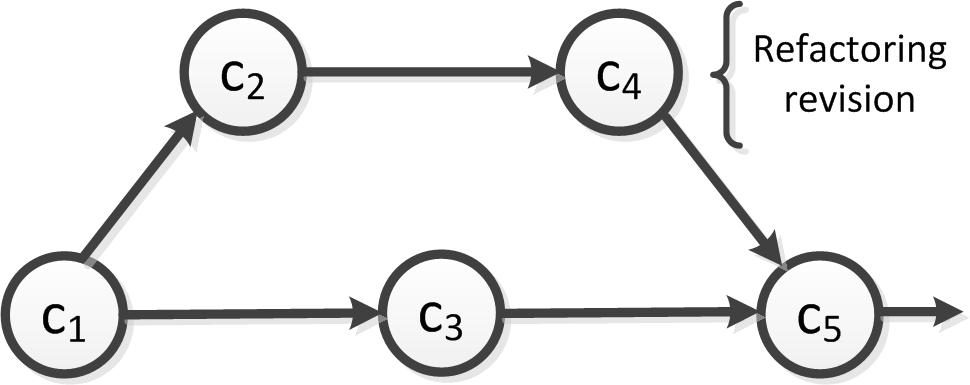
\includegraphics[width=2.5in]{../img/implicit_branche}
	\caption{Exemplo de implicit branches \cite{Tsantalis2013}{}.}
	\label{fig:implicit_brache}
\end{figure}

As refatorações foram detectadas utilizando a técnica proposta Tsantalis et al. \cite{Tsantalis2013}{} que é baseada no algoritmo \texttt{UMLDiff} \cite{Xing:2005:UAO:1101908.1101919}. Tendo em vista a ausência de código compilado foi utilizado uma implementação da técnica com algumas adaptações \cite{Danilo}. A ferramenta proposta Tsantalis et al. é capaz de detectar  11 tipos diferentes de refatoração. Para a refatoração Mover Classe a detecção ocorre com base nas seguintes regras conforme definidas por \cite{Biegel:2011:CSM:1985441.1985452}:
\begin{itemize}
	\item Seja $(p,n,m)$ uma tupla tal que $p$ é o pacote que uma classe pertence, $n$ é o nome da classe e $m$ é o conjunto de métodos e campos que compõe a classe.
	\item Seja $t$ que corresponde uma comparação entre duas revisões sucessivas
	\item Seja $C^{+}_{t}$ o conjunto de classes adicionadas na transação $t$
	\item Seja $C^{-}_{t}$ o conjunto de classe removidas na transação $t$
	\item A refatoração é detectado quando as duas condições a seguir são verdadeiras:
		\begin{itemize}
			\item $\exists (p,n,m) \in C^{-}_{t}$
			\item $\exists (p^{'},n,m) \in C^{+}_{t}$
		
		\end{itemize}
\end{itemize}

Em resumo a detecção da movimentação das classes consiste em verificar se uma classe que previamente existe um em pacote $p$ em uma versão $v_{1}$ está no pacote $p^{'}$ na versão subsequente $v_{2}$. No estudo empírico de \cite{Tsantalis2013} foi verificado um número baixo de falsos positivos e por consequência uma alta precisão quando utilizado este conjunto de regras na detecção de Mover Classe.

\subsubsection{Seleção dos \texttt{batching moving} }

Conforme a definição proposta neste trabalho, um  \texttt{batching moving} representa uma movimentação de classe em um número maior do que padrão do sistema. Desta forma, para detectamos este tipo de evento foi necessário avaliar a frequência que a refatoração Mover Classe ocorre nos sistemas em estudo. Neste estudo foi definido que a ocorrência de \texttt{batching moving} é determinada por um total de classe movimentadas que é maior o igual 1.5 vezes a média de ocorrência da refatoração Mover Classe no sistema.  A Tabela \ref{tab:visao-geral} exibe os valores da média, mediana e desvio padrão da distribuição de Mover Classe entre diferente versões dos sistemas. A coluna \textit{Valor do batching moving} apresenta o valor de referência utilizado para detectar movimentações de classes atípicas no sistema.
% Please add the following required packages to your document preamble:
% \usepackage{graphicx}
\begin{table}[]
	\centering
	\resizebox{\textwidth}{!}{%
		\begin{tabular}{|c|c|c|c|c|c|}
			\hline
			\textbf{Projeto} & \textbf{Total} & \textbf{Média} & \textbf{Mediana} & \textbf{Desvio Padrão} & \textbf{Valor do batching moving} \\ \hline
			clojure          & 64             & 15,5           & 2                & 23,08                  & 23                                \\ \hline
			gradle           & 4253           & 31,3           & 2                & 12,9                   & 46                                \\ \hline
			junit4           & 279            & 12             & 2                & 7,9                    & 18                                \\ \hline
			spring-framework & 1427           & 26             & 2                & 12,5                   & 39                                \\ \hline
		\end{tabular}%
	}
	\caption{Media, Mediana, Desvio Padrão e Valor do batching moving}
	\label{tab:visao-geral}
\end{table}



\subsection{Análise das Mensagens de Commit}
\label{subsec:analise_commit}

Com o objetivo de analisar se os desenvolvedores reportam que a refatoração Mover Classe teve como objetivo alterar a arquitetura do sistema, foi realizada uma inspeção manual nas mensagens dos commits. Foi avaliado aqueles commits que movimentaram classe um número maior do que 1.5 vezes a média do sistema. Na busca foi avaliado a existência de evidências que a refatoração visava melhorar algum atributo interno do sistema ou ainda adequar a alguma arquitetura previamente definida. 

%\subsection{Pesquisas com os Desenvolvedores}
%\label{subsec:pesquisas_desenvolvedores}


\section{Resultados}
\label{sec:resultados}

Neste seção apresentados os resultados para as questões de pesquisas propostas. Em resumo, este estudo avaliou um total de 52001 diferentes versões de sistemas, do qual foi possível detectar o montante de 35402 refatorações diferente. Do total de refatorações encontrados 17\% era do tipo Mover Classe. A coluna \textit{Mover Classe} exibe o número da refatoração em estudo, bem como o seu percentual, para cada sistema.  A Tabela \ref{tab:estatisticas} detalha estes número para cada projeto.


% Please add the following required packages to your document preamble:
% \usepackage{graphicx}
\begin{table}[htb]
	\centering
	\resizebox{\textwidth}{!}{%
		\begin{tabular}{|c|c|c|c|}
			\hline
			\textbf{Projeto} & \textbf{\#Commits} & \textbf{\#Refactorings} & \textbf{\#Mover Classe} \\ \hline
			clojure & 2923 & 522 & 64 (12,3\%) \\ \hline
			gradle & 35593 & 20258 & 4253 (21\%) \\ \hline
			junit4 & 1721 & 1070 & 279 (26,1\%) \\ \hline
			spring-framework & 11764 & 13552 & 1427 (10,5) \\ \hline
			Total & 52001 & 35402 & 6023 (17\%) \\ \hline
		\end{tabular}%
	}
	\caption{Estatísticas dos Sistemas Analisados}
	\label{tab:estatisticas}
\end{table}

\subsection{Com qual frequência a refatoração Mover Classe tem por objetivo alterar a arquitetura do sistema (\texttt{batching moving})?}

As Figuras \ref{fig:resultado-clojure}, \ref{fig:resultado-gradle}, \ref{fig:resultado-junit}, \ref{fig:resultado-spring} exibem a frequência e o número de ocorrência da refatoração Moves Classe. Por exemplo, na Figura \ref{fig:resultado-clojure} é possível verificar a ocorrência de uma refatoração do tipo Mover Classe onde um total de 54 itens foram movidos. A linha tracejada na horizontal representa o valor acumulado da frequência da refatoração estudada. Por outro lado, a linha contínua na horizonte refere-se ao valor limite para determinação de um \texttt{batching moving}. Neste exemplo, temos que apenas uma única vez para o sistema \texttt{clojure} ocorreu uma movimentação de classe acima do padrão. 

\begin{figure}[ht]
\centering
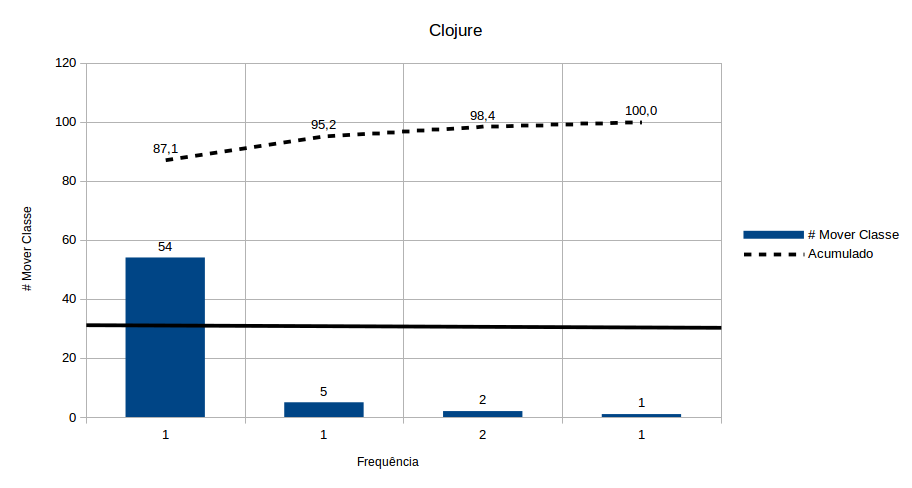
\includegraphics[width=0.9\linewidth]{../img/results-clojure}
\caption[Frequência de Mover Classe]{}
\label{fig:resultado-clojure}
\end{figure}

\begin{figure}
	\centering
	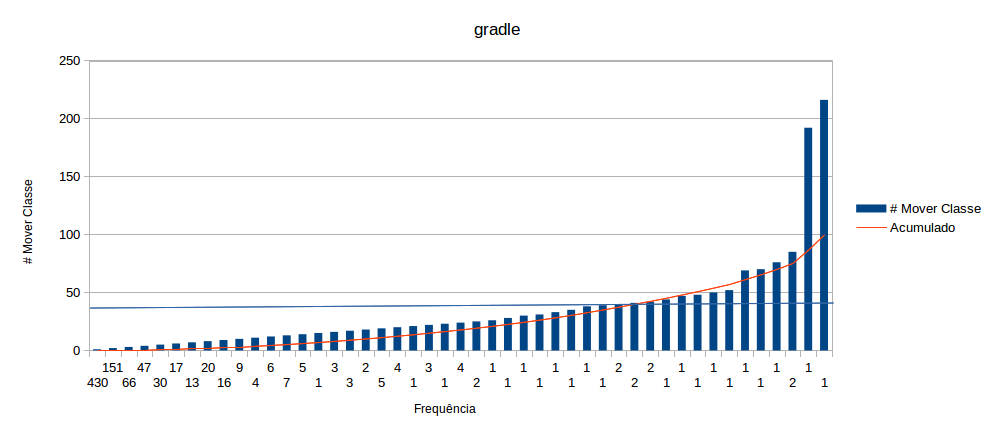
\includegraphics[width=0.9\linewidth]{../img/results-gradle}
	\caption[Frequência de Mover Classe]{}
	\label{fig:resultado-gradle}
\end{figure}


\begin{figure}
	\centering
	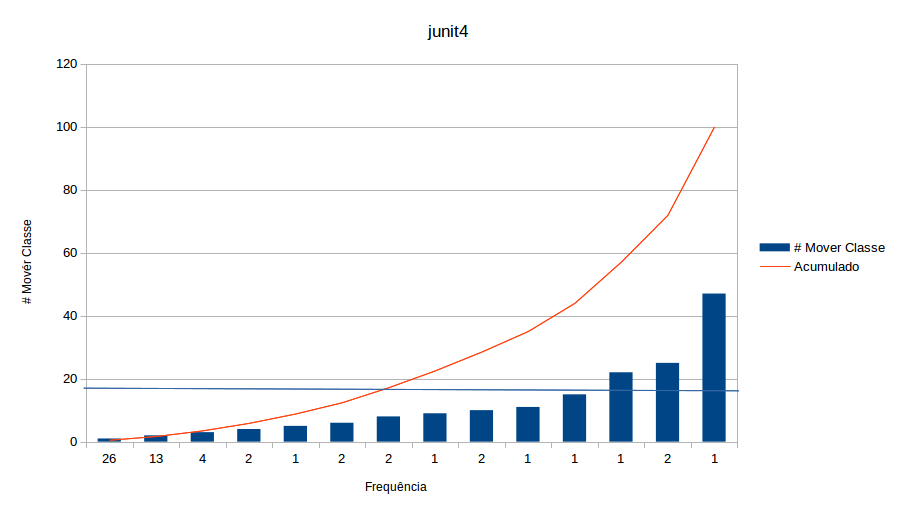
\includegraphics[width=0.9\linewidth]{../img/results-junit}
	\caption[Frequência de Mover Classe]{}
	\label{fig:resultado-junit}
\end{figure}

\begin{figure}
	\centering
	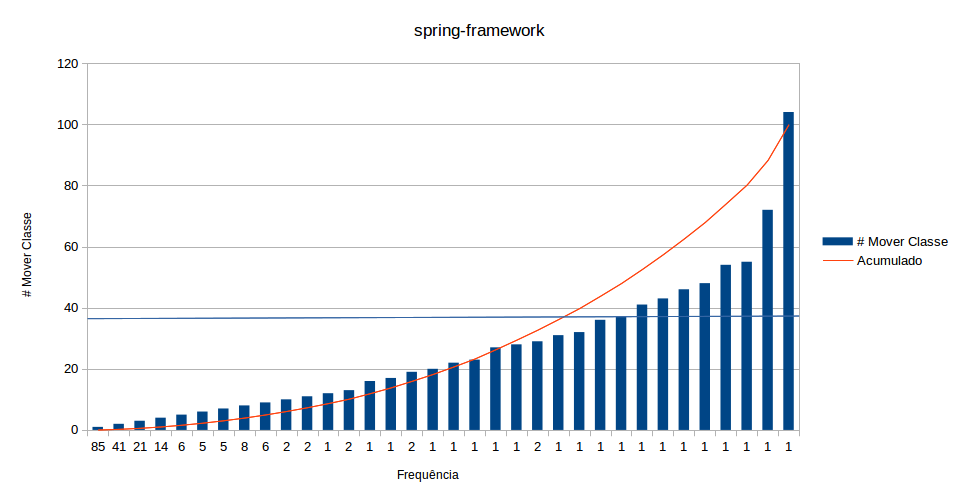
\includegraphics[width=0.9\linewidth]{../img/results-spring}
	\caption[Frequência de Mover Classe]{}
	\label{fig:resultado-spring}
\end{figure}




\section{Ameaças à Validade}
\label{sec:ameacas}

\section{Trabalhos Relacionados}
\label{sec:trabalhos-relacionados}

\section{Conclusão}
\label{sec:conclusao}
\bibliographystyle{sbc}
\bibliography{../bib/paper-arqsw}

\end{document}
